\documentclass{article}
\usepackage[UTF8]{ctex}
\usepackage{geometry}
\usepackage{natbib}
\geometry{left=3.18cm,right=3.18cm,top=2.54cm,bottom=2.54cm}
\usepackage{graphicx}
\pagestyle{plain}	
\usepackage{setspace}
\usepackage{caption2}
\usepackage{datetime} %日期
\renewcommand{\today}{\number\year 年 \number\month 月 \number\day 日}
\renewcommand{\captionlabelfont}{\small}
\renewcommand{\captionfont}{\small}
\begin{document}

\begin{figure}
    \centering
    
\includegraphics[width=8cm]{upc.png}

    \label{figupc}
\end{figure}

	\begin{center}
		\quad \\
		\quad \\
		\heiti \fontsize{45}{17} \quad \quad \quad 
		\vskip 1.5cm
		\heiti \zihao{2} 《计算科学导论》课程总结报告
	\end{center}
	\vskip 2.0cm
		
	\begin{quotation}
% 	\begin{center}
		\doublespacing
		
        \zihao{4}\par\setlength\parindent{7em}
		\quad 

		学生姓名:\underline{\qquad  吴晓云 \qquad \qquad}

		学\hspace{0.61cm} 号:\underline{\qquad 1907010201\qquad}
		
		专业班级:\underline{\qquad 计科1901 \qquad  }
		
        学\hspace{0.61cm} 院:\underline{计算机科学与技术学院}
% 	\end{center}
		\vskip 2cm
		\centering
		\begin{table}[h]
            \centering 
            \zihao{4}
            \begin{tabular}{|c|c|c|c|c|c|c|}
            % 这里的rl 与表格对应可以看到,姓名是r,右对齐的;学号是l,左对齐的;若想居中,使用c关键字。
                \hline
                课程认识 & 问题思 考 & 格式规范  & IT工具  & Latex附加  & 总分 & 评阅教师 \\
                30\% & 30\% & 20\% & 20\% & 10\% &  &  \\
                \hline
                 & & & & & &\\
                & & & & & &\\
                \hline
            \end{tabular}
        \end{table}
		\vskip 2cm
		\today
	\end{quotation}

\thispagestyle{empty}
\newpage
\setcounter{page}{1}
% 在这之前是封面,在这之后是正文
\section{引言}
计算科学导论的定位是高级科普,目的在于让计算机科学与技术领域的初学者了解专业技术知识。计算科学导论很少涉及具体的专业知识,它只是对未来学习专业知识的一个导引。对于以后将会学习到的专业名词与方法等进行介绍,重在引导初学者怎么从科学哲学的角度去认识和学习计算科学,当然,也包括为学习后续课程准备的布尔代数基础知识。学习这门课,不需要完全懂得其中所包括的内容,只需要大体理解,具体的内容在以后的学习中会逐步学习,具体学习。\par
导论中许多的观点和思想方法对我们以后的大学生活中有很大的作用,比如其中所涉及的学科方法论,这对我们以后学习各个学科有很大作用。


\section{对计算科学导论这门课程的认识、体会}
\par

\subsection{对计算科学导论这门课程的认识、体会}
从20世纪30年代到60年代初,计算机科学与技术的研究与学科发展基本上是处在萌芽阶段,当时从事计算机科学与技术研究的科学家主要来自数学和电子科学领域。20世纪50年代后期高级程序设计语言的发展促进了硬件、软件与理论的融合,计算的数学理论等多个方向的研究进展催生了计算机科学与技术作为一个学科的出现。到了70和80年代,众多大学的计算机科学系逐步分化为计算机科学系和计算机工程系等两大阵营,以后又出现了一些变形。在1989年,联合攻关小组提交并发表了《计算作为一门学科》的研究报告,认为计算机科学系和计算机工程系没有区别,本质相同。\par
在中国,其研究始于20世纪50年代,中国科学院开始培养学科专业技术人才。从70年代初起,一些学校的数学系开始设置计算机专业。至80年代中期,逐步将专业更名为计算机科学理论、计算机软件、计算机系统与结构等等。最后,在90年代后期又进行了一次调整,本科专业统一为计算机科学与技术,研究生则继续保留软件与理论。体系结构、计算机应用技术三个专业。\par
“近年来,计算机技术取得了飞速的发展。在较短的时间 内,人们对计算机的需求还会不断增加”,“计算机技术是社会发展的必然趋势”,在杨成雄发表的期刊《浅议计算机科学技术的现状及发展前景》\citep{yangchengxiong}中展示了计算机科学与技术的发展趋势。\par



\subsection{计算科学的意义及基本问题}
计算科学是对描述和变换信息的算法课程,包括其理论、分析、设计、效率分析、实现和应用的系统的研究。计算不等于数学,但数学起源于对计算的研究。\par
基本问题:\par
(1)计算的平台与环境问题:不是所有的计算模型都能运行,只有构造性计算模型才是有可能运行的。但是,并不是凡是具有能行性特点的计算模型都能够造出具体的自动计算设置,如非确定性计算模型。\par
(2)计算过程的能行操作与效率问题:一个问题在判明为可计算的性质后,从具体解决而这个问题着眼,必须按照能行可构造的特点与要求,给出实际解决该问题的一步一步的具体操作,同时还必须确保这样一种过程的开销成本是我们能够接受的。\par
(3)计算的正确性问题:这是任何计算工作都不能回避的问题,特别是使用自动计算机器进行的各种计算。一个计算问题再给出能行操作序列的同时,必须确保计算的正确性,否则,计算是无意义的。\par



\subsection{计算机科学与技术体系核心内容}
计算机科学与技术课程体系包含的内容有很多,其中其核心内容是:计算机语言程序设计,例如C语言,C++等,它们就是计算机能识别的程序设计语言;数据结构,数据结构和算法是程序的根本,好的数据结构可以使程序更加高效率的运行;计算机组成与结构;操作系统,它是配置在计算机上的第一层软件,它的性能能直接影响计算机系统的工作效率;编译原理;数据库系统,差不多所有的软件系统都需要数据库的支持;离散数学;还有软件工程、计算机网络、面向对象的程序设计计算机图形学等等。\par
\subsection{计算科学给我的思考及体会}
导论除了介绍了计算机组织与结构、高性能计算等基本知识,还让我从更高的高度看待事物,也是拓展了我的视野。老师在上课时结合了很多如今的实例,让我了解到更多。在此之前,其实我对计算机科学与技术的了解很浅显,只知道是学计算机,具体有什么都不知道,但在学了计算科学导论后,我有了大体的框架,大致了解了这个专业,大致知道以后会学到的东西。当然,最重要的是,通过分组报告和研读课本,我也知道了以后的职业方向,知道用到计算机的职业。另外,计算科学导论这本书真的很有用,尤其是对以后,每读一遍都有一遍的收获,当然了,我现在只读了一遍,但是我相信,等我大三大四再读,得到的一定会比现在多。\par
还有一点,我印象很深的,仍记得老师说的“从事这个行业就是要不断的学习,每天学习”,时刻更新自己的知识见闻,因为计算机这个行业更新太快了,一段时间不学,就跟不上发展,只有不停的学习才能保证跟上发展更新脚步,不被淘汰。\par



\section{进一步的思考}
本次分组报告,我的课题是智慧银行,在演讲之后,我有以下补充:\par
1、	智慧银行应用了哪些技术:区块链技术、大数据、5G应用、物联网、人工智能等。\par
2、	智慧银行中应用的这些技术分别是如何应用的:\par
区块链技术:区块链技术是使用密码学并通过不同算法产生新的数据块,每一个数据块中包含过去约定时间内所有的交易信息,验证信息的有效性和生成下一个区块。应用区块链技术提高的信息可靠性。区块链技术通过建立去中心化的信用创造方式解决“拜占庭将军问题”,即确定一套算法,通过技术背书而非中心化信用机构来进行信用创造。但是,从期刊《A framework for analysing blockchain technology adoption: Integrating institutional, market and technical factors》\citep{qukuailian},其中的“The adoption of blockchain technologies require the consideration of a broad range of factors, over and above the predominantly technology focus of most current work. ”我们能了解到,应用区块链技术还有很长的路要走。\par
大数据:大数据增强了银行营销的精准性,提高了网点运营管理能力与银行风险的防控能力。360度视图及画像、营销模式实验室、营销过程管理平台与如影随形的业务移动都应用了大数据。
分开来说,在支持精准营销方面,利用大数据分析挖掘方法建立完善的产品响应体系,支持精准营销策略的智能化运作,持续提升产品推荐的智能性和精准性。在支持风险识别方面,加快人工智能技术在风险管理领域的应用,预判风险客户违约概率,并对风险客户进行预警提示;研发基于大数据的个人客户贷前、贷中、贷后预警模型;制定更为精细化的信用卡授信策略,完善信用卡业务及风险监测预警模型体系。在支持绩效考核方面,完善客户贡献评价标准,实现客户贡献模型的显性化、可视化、集成化和标准化。在支持市场拓展方面,充分利用工商注册企业信息、海关、征信信息、移动APP、位置信息等外部数据或客户关系信息支持新客户拓展,探索基于互联网客户需求的直销式获客,创造新的客户来源。
我们就可以在这几个方面,根据自己所感兴趣的,选择将来就业方向。\par
5G应用:将5G运用于全球专家连线、远程客服等场景中,可以通过VR进行面对面交流,以5G技术为基础,将生物识别、人工智能、物联网、全息投影、VR、大数据等新科技,应用于迎宾识别、互动体验、展示销售、业务办理等客户全旅程服务。很多对5G感兴趣的,就可以在这几个方面寻找就业岗位。\par
物联网:“Physical world integration with cyber world opens the opportunity of creating smart environments; this new paradigm is called the Internet of Things (IoT).”期刊《Challenges and recommended technologies for the industrial internet of things: A comprehensive review》\citep{wulianwang}这样介绍物联网。物联网可以应用于现金管理,通过物联网可以直接定位钞箱,押运车的运行轨迹以及范围,可以实现对现金运输过程中的安防管理以及及时跟踪。在现金运输流动环节遇到突发状况时,可以迅速启动应急预案,及时通知监管人员、安保部门,甚至公安人员,同时进行图像以及声音采集及时传输,便于相关人员更好处理事件,同时也可发出警报声震慑不法分子。还通过物联网技术管理固定资产设备。利用系统给固定资产建立独立的电子标签。\par
人工智能:一些国际监管机构,例如澳大利亚证券及投资委员会(ASIC)、新加坡货币当局(MAS)及美国证券交易委员会(SEC),都在使用人工智能进行可疑交易识别。还用于银行的人脸识别。得益于人工智能算法带来的图像识别率上升,OCR(Optical Character Recognition,光学字符识别技术)技术可以将原来前台分散进行的证件审核、银行卡识别、票据审核、票据录入等人工操作转移到后台运营中心进行,不仅效率提升,而且风控措施也得到了增强,语音识别、自然语言理解技术的采用,使本已经实现集中化运营的客服中心进一步降低了人员需求,这些都应用了人工智能。\par
“展望未来,建设以科技引领的 智慧银行是大势所趋,在应用新兴 技术和工具的同时,运营与管理架 构也应不断革新适应,银行需要制 定具有前瞻性、全局性、系统性的 金融科技发展战略,探索适合自身 发展的智慧银行建设路径,开启银行高质量发展的新征程”在中一禾发表的期刊《共建开放生态,打造智慧银行》\citep{zhongyihe}中对技术对于智慧银行的重要性进行了阐述。\par
当然,智慧银行中所应用的技术绝不仅有这五个,还有很多其他的技术。若对这其中的技术有兴趣,可以把它作为一个将来就业行业的考虑方向。\par




\section{总结}

计算机科学导论是学习计算机知识的入门知识,同时也是我们计算机专业的核心课程之一。计算科学导论是对计算机领域专业知识的高级科普书,从计算科学一词的来历入手,进行之后内容的介绍。通过通俗流畅的语言,像我们介绍了以后将会学到的知识。这本书就像高雅艺术,不需要我们面面俱到的掌握理解它,只需要我们连接以后将会学习到的东西,并进一步认识计算机科学与技术,知道如何学习计算机科学与技术问题,帮助我们接下来专业知识的学习。\par
尽管这门课程不要求掌握很深刻的东西,但是我从此次课程中学到了很多东西。例如,第二章讲计算科学的基本概念和基础知识,这一章介绍了计算模型与二进制,数字逻辑与集成电路,汇编语言,算法等等,其中,我在学习这门课以前,并不知道汇编语言这个名词,而在我学习完之后,我不仅知道了汇编语言是什么,还知道为什么这种语言虽然在可读性和编写程序时不能令人满意,但至今仍有不少工程师在系统软件的开发中使用它。当然,除了课本本身带给我的东西之外,还能根据他所介绍的东西,找到自己所感兴趣的,然后查找资料,更深入的去了解。比如,在介绍了图灵机之后,引发了我的兴趣,于是我阅读了赵正平的一篇论文《图灵机及其构造研究》\citep{zhaozhengping},更进一步的了解了图灵机的结构,然后,又通过期刊论文《基于量子逻辑的图灵机及其通用性》\citep{liping}了解了一种特殊的图灵机--通用图灵机。\par
由此可见,计算科学导论这门课对我们的影响绝不局限于课本。
同时,导论还在通识教育观下,引导初学者具备高素质人才的条件: \par
(1)具有高尚的品德和良好的人文素养。 \par
(2)具有坚实的专业基础和深厚的专业功底。 \par
(3)具有创新意识,具有科学的思想方法。 \par


\section{附录}
\begin{itemize}
    \item 申请Github账户,给出个人网址和个人网站截图
    \begin{figure}[h!]
    	\centering
    	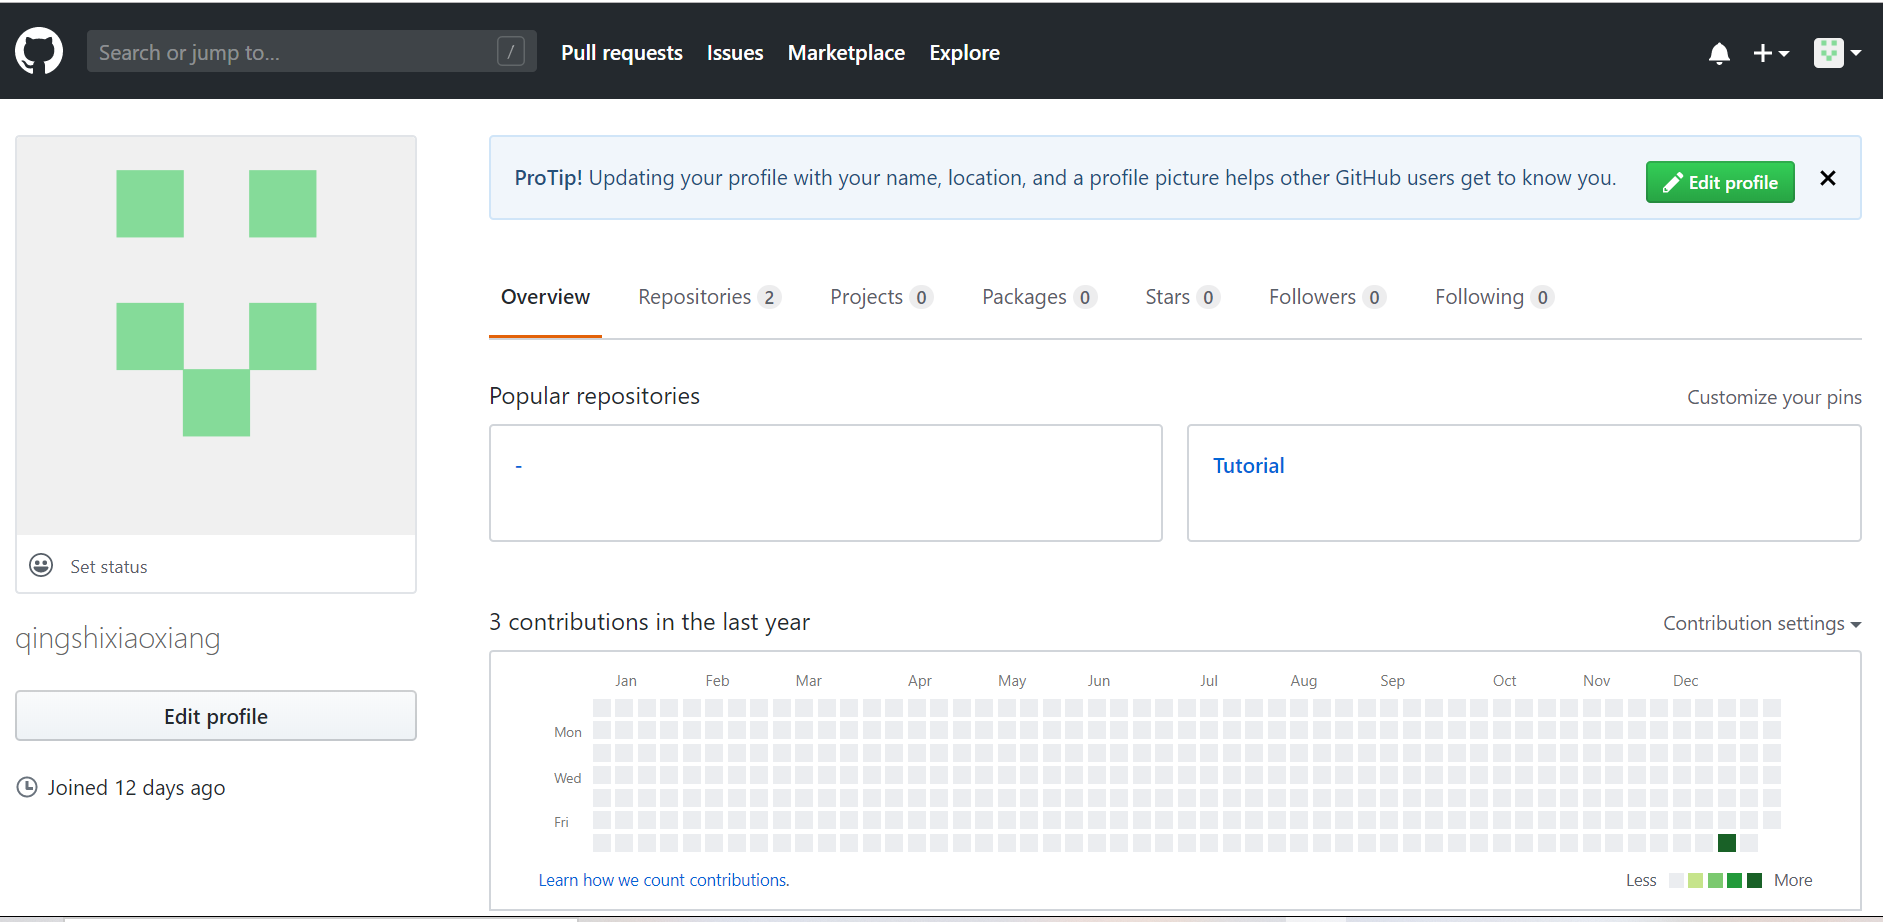
\includegraphics[scale=0.25]{github}
    	\label{fig:github}
    	\caption{Github}
    \end{figure}
    \item 注册观察者、学习强国、哔哩哔哩APP,给出对应的截图
    \begin{figure}[h!]
    \centering
    
\includegraphics[scale=0.35]{guanchazhe}
    \label{fig:guanchazhe}
    \caption{观察者}
    \end{figure}
    \begin{figure}[h!]
    \centering
   	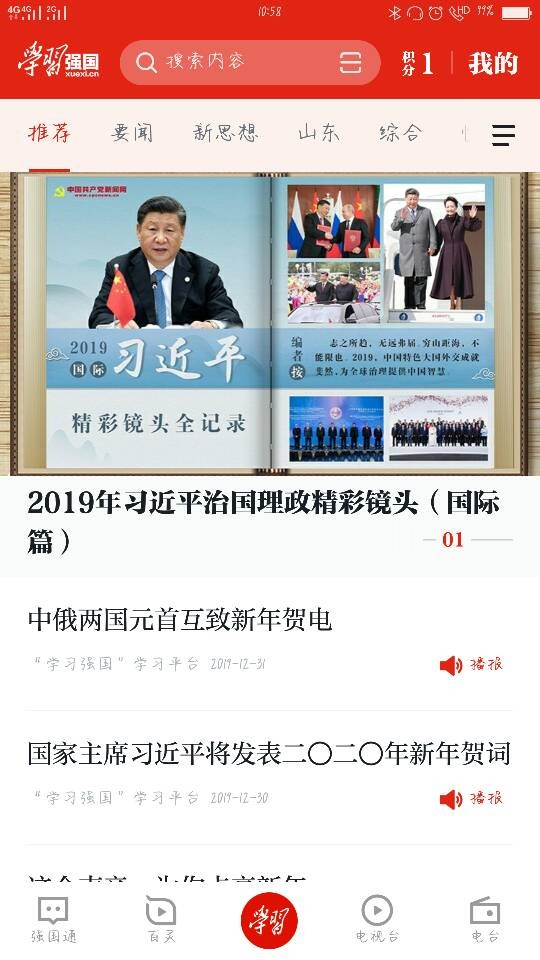
\includegraphics[scale=0.25]{xuexiqiangguo}
   	\label{fig:xuexiqiangguo}
   	\caption{学习强国}
    \end{figure}
    \begin{figure}[h!]
	\centering
	\includegraphics[scale=0.25]{bilibili}
	\label{fig:bilibili}
	\caption{哔哩哔哩}
    \end{figure}
    \item 注册CSDN、博客园账户,给出个人网址和个人网站截图
    \begin{figure}[h!]
    	\centering
    	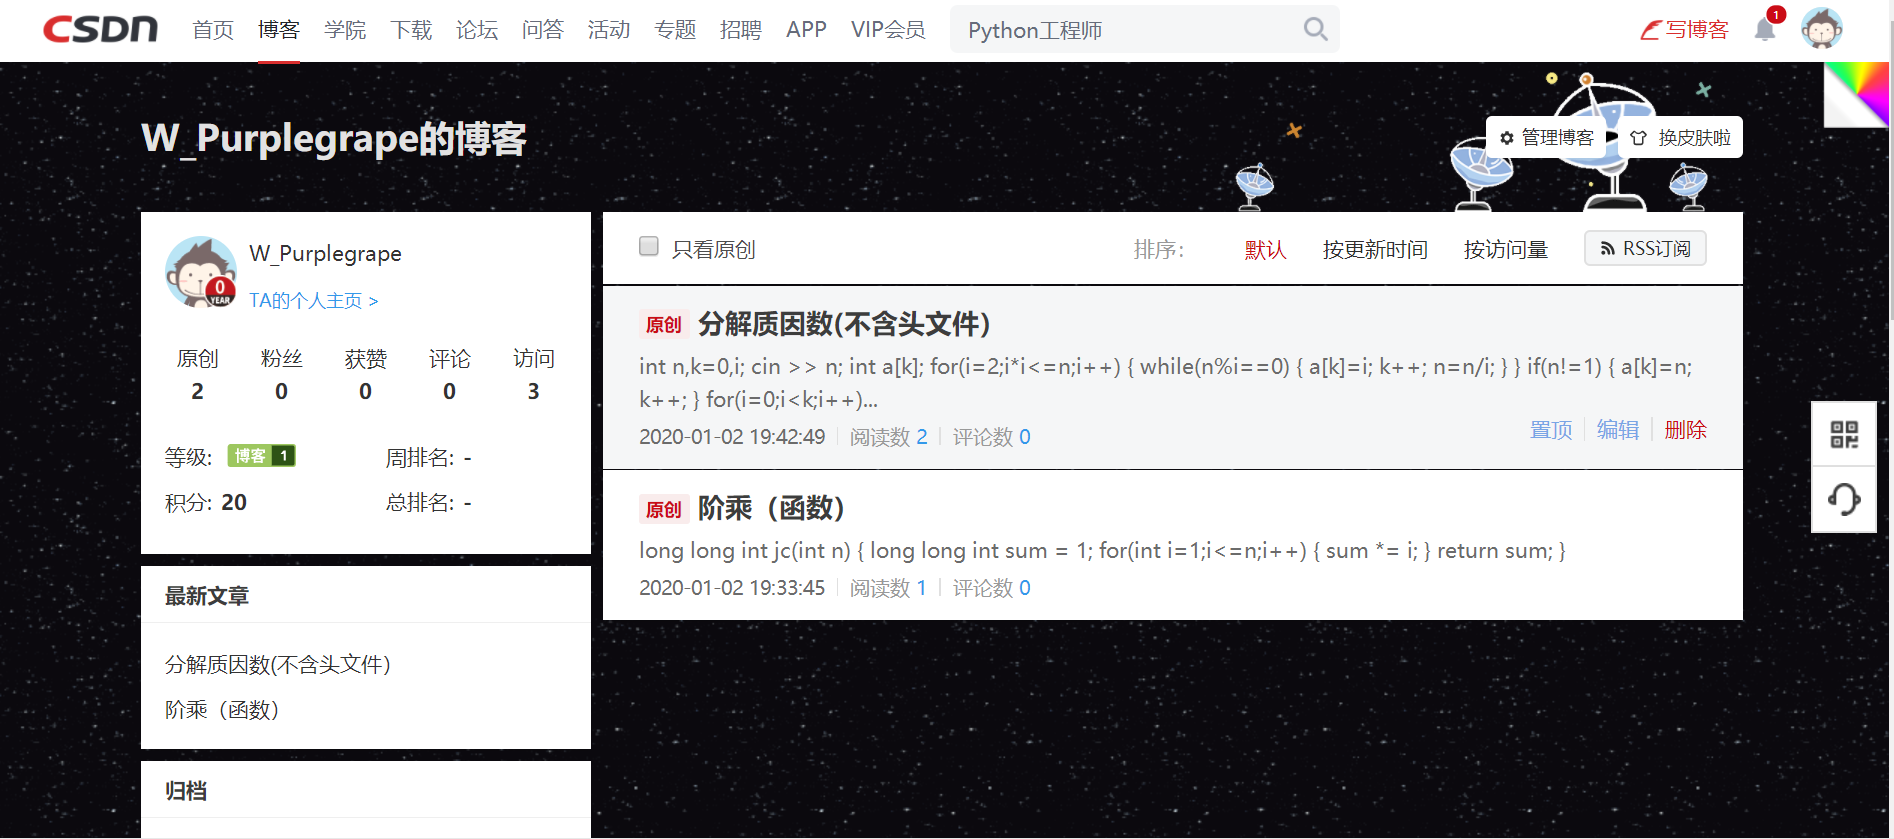
\includegraphics[scale=0.25]{csdngeren}
    	\label{fig:csdngeren}
    	\caption{CSDN个人网站}
    \end{figure}

\begin{figure}[h!]
	\centering
	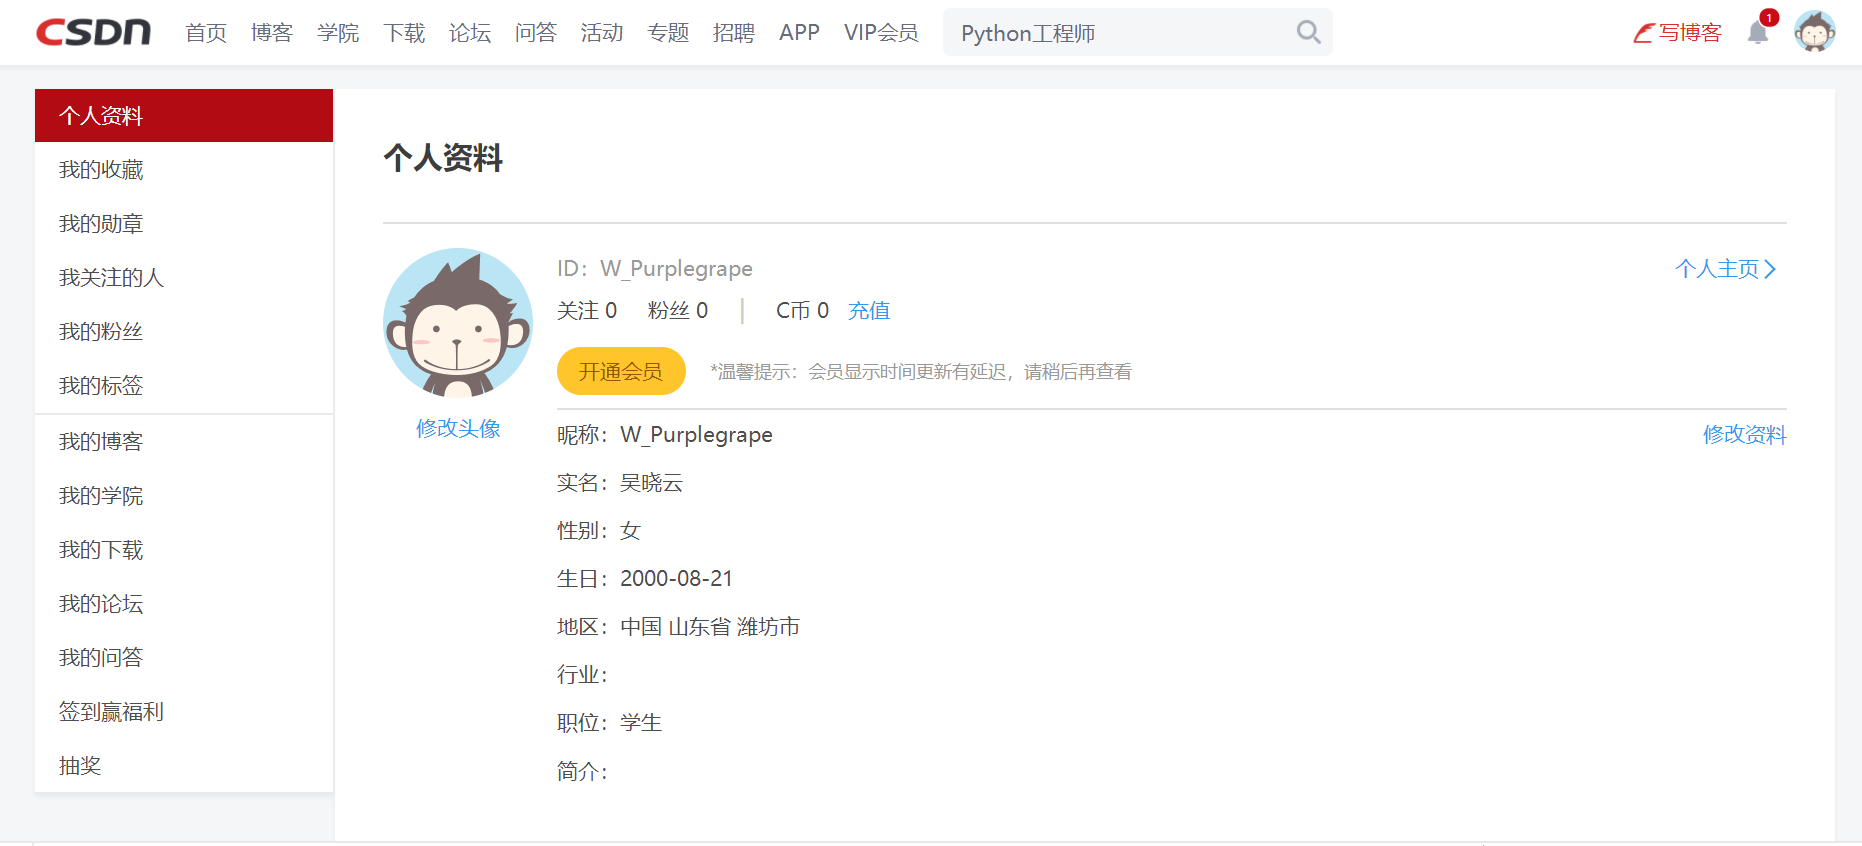
\includegraphics[scale=0.25]{csdnwangzhan}
	\label{fig:csdnwangzhan}
	\caption{CSDN个人主页}
\end{figure}
\begin{figure}[h!]
\centering
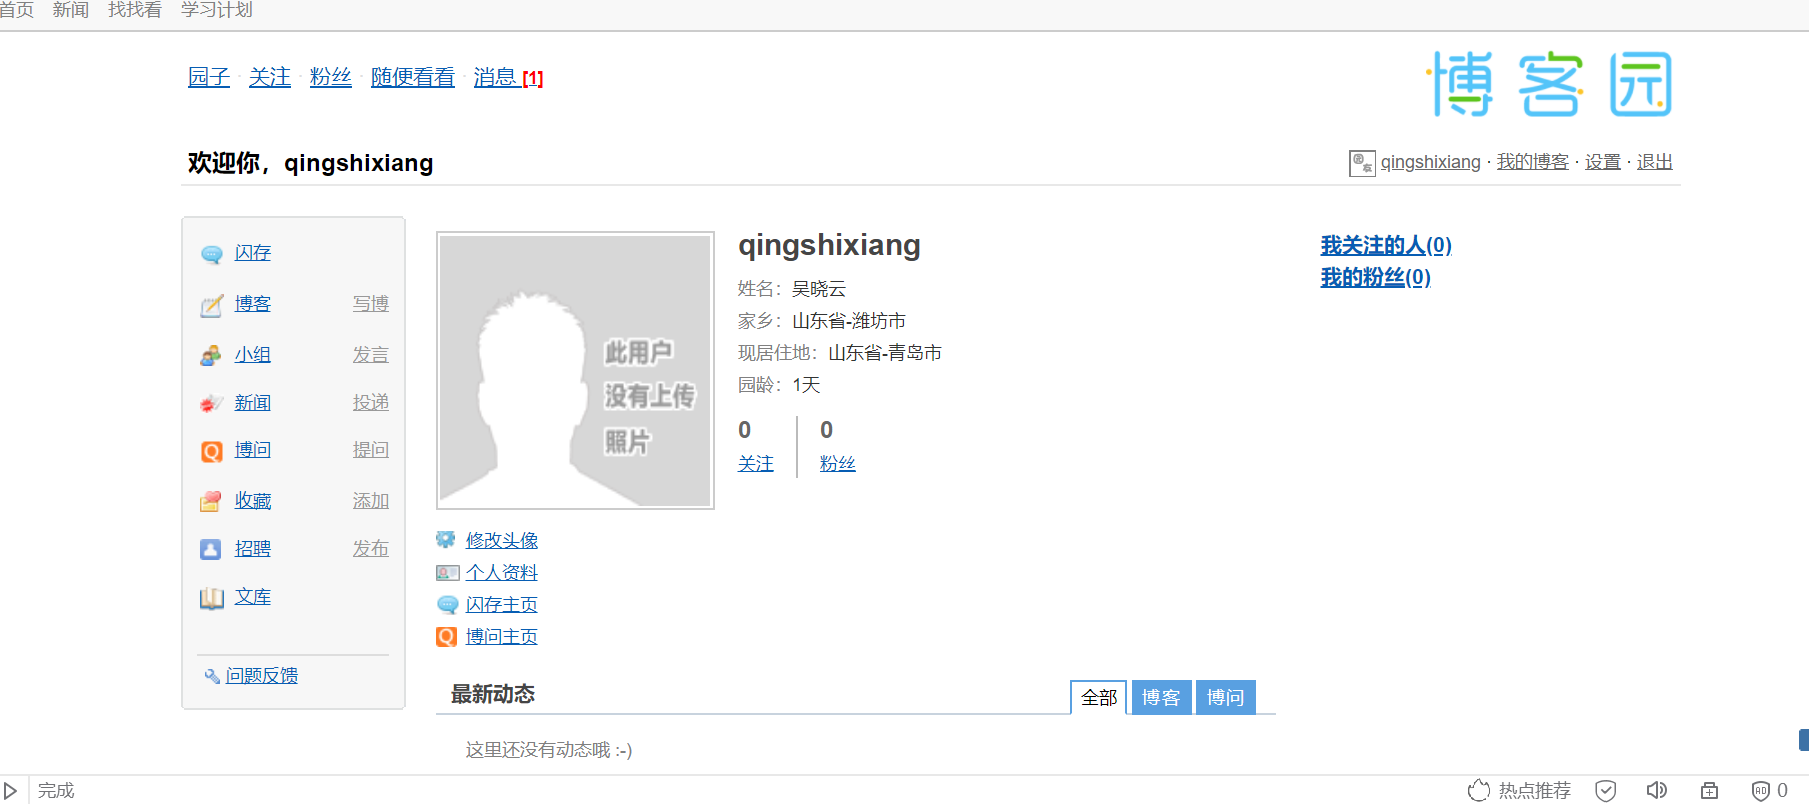
\includegraphics[scale=0.25]{bokeyuangeren}
\label{fig:bokeyuangeren}
\caption{博客园个人主页}
\end{figure}
\begin{figure}[h!]
	\centering
	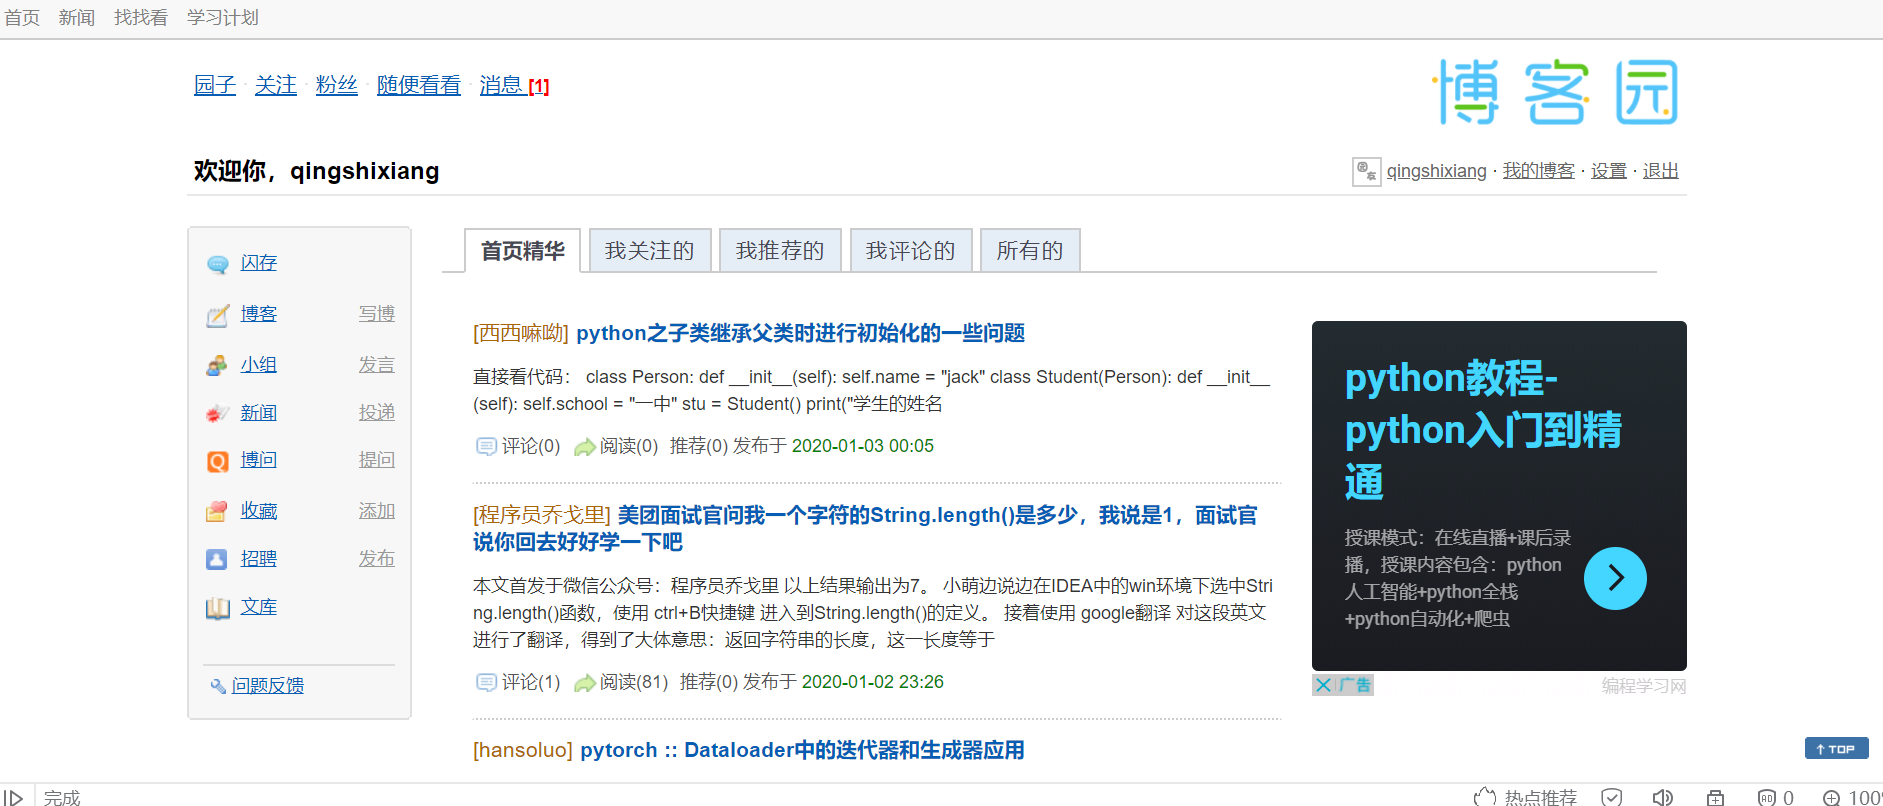
\includegraphics[scale=0.25]{bokeyuanwangzhan}
	\label{fig:bokeyuanwangzhan}
	\caption{博客园网站}
\end{figure}
    \item 注册小木虫账户,给出个人网址和个人网站截图
    \begin{figure}[h!]
    	\centering
    	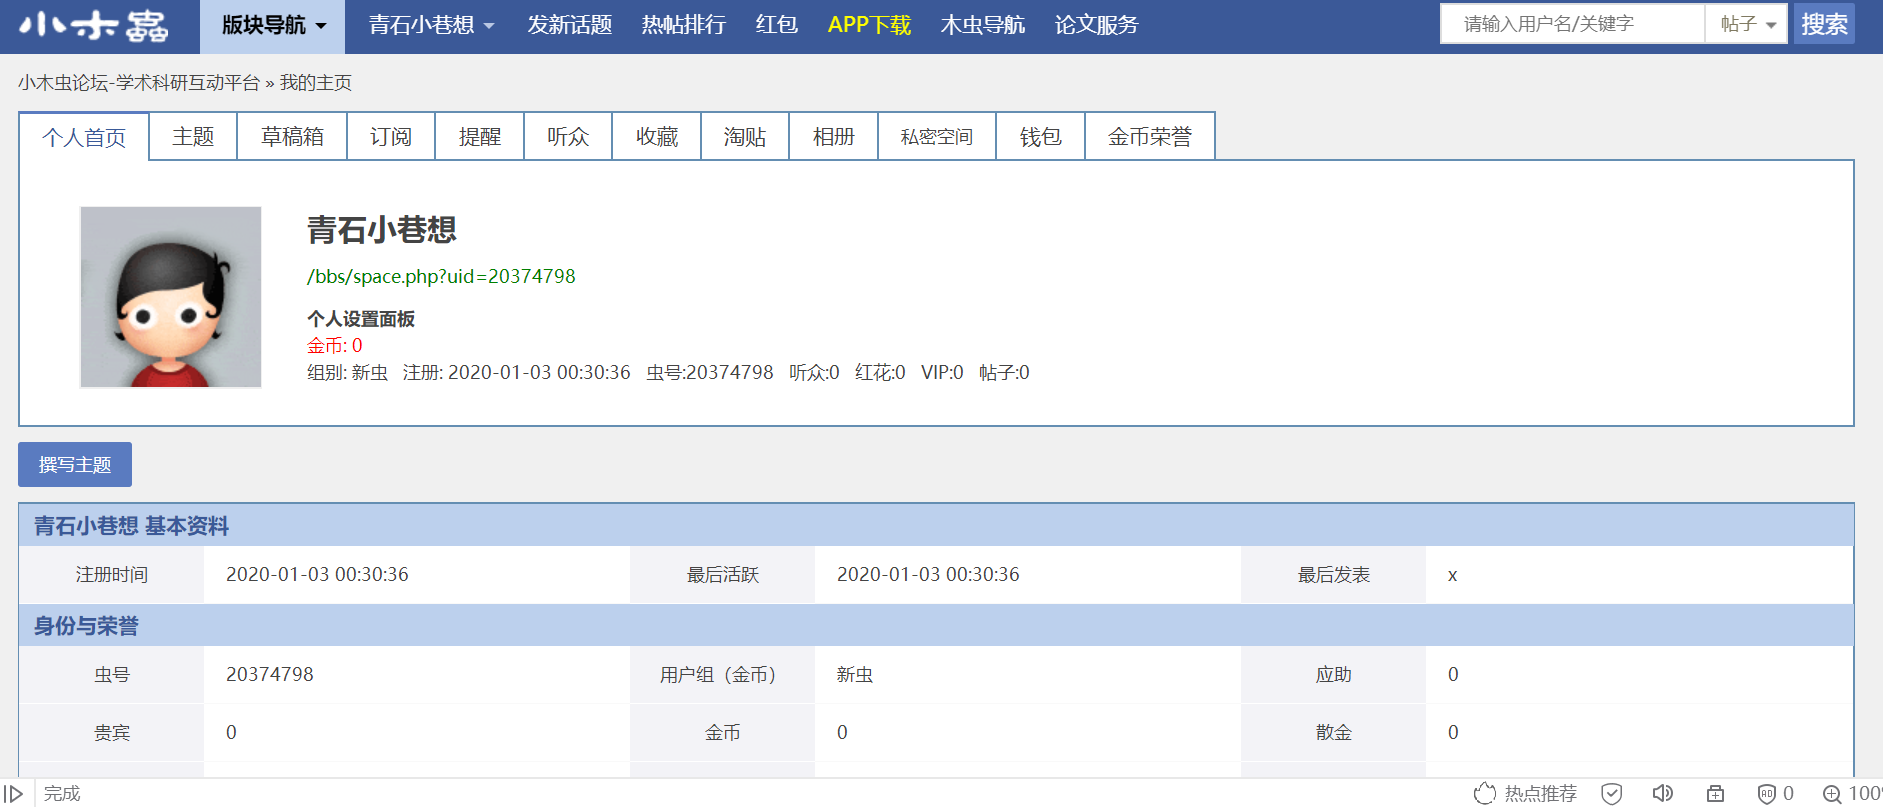
\includegraphics[scale=0.25]{xiaomuchonggeren}
    	\label{fig:xiaomuchonggeren}
    	\caption{小木虫个人主页}
    \end{figure}
\end{itemize}

\hspace*{\fill} \\

\bibliographystyle{unsrt}
\bibliography{cankao}




\end{document}
